\section{Investigation of effects of varying scoring weights}
\label{sect:exp_scoring}
\subsection{Introduction}

This investigation involves running a series of one-night simulations under different environmental assumptions to see the effect of varying the relative values of the scoring heuristic weights. The rational behind this investigation is to provide some initial insight into the usefulness of the various \emph{Schedule Quality Metrics} (SQM) and to provide a shakedown test of the simulation framework on real data. By selecting 2 seperate but similar nights (in terms of loading) it should be possible to get a preliminary idea on the range of likely values and variation of these metrics.


\subsection{Method}
Two nights were considered and are detailed in Table.~\ref{tab:scoring_nights}. On night \emph{$^\#$1} (27th-28th September 2007), the moon rises early and is up for the full night. There are  12 hours of night of which 9.5 hours are astronomically dark. Night \emph{$^\#$2} (3th-4th November 2007) has 5.5 hours of lunar dark time at the start of the night during the 13.0 hour night of which 10.2 hours are astronomically dark.

 A series of simulations were run for fixed environmental scenarios $E_{FX}$ (fixed, excellent seeing) and $E_{FP}$ (fixed, poor seeing) on each of the two nights. The scoring model was chosen to be:-

\begin{equation}
\label{eq:two_score}
  f_g = w_{trans} f_{trans}(g,t,E) + w_{px} f_{px}(g,t,E)
\end{equation}

The weights of the \emph{transit elevation} function $w_{trans}$ and the \emph{execution priority} function $w_{px}$ were varied for each set of 1000 simulations such that $w_{trans} + w_{px} = 1$. These two functions were chosen as they are generally (operationally) the highest weighted functions and because $f_{px}$ does not vary in time whereas $f_{trans}$ does vary with time for a given group. No other functions were incorporated into the scoring calculation in order to avoid any unnecessary noise.

The SQMs used to evaluate the quality of the resulting schedules are $Q_{OA}$ - the optimal airmass metric, $Q_{PX}$ - the execution priority metric, $Q_{RN}$ - urgency metric, $Q_{TD}$ - demand metric, $Q_{PX \cdot OA}$ - priority weighted optimal airmass and $Q_{XT}$ the total execution time as a fraction of available night. 

In addition, for each set of simulation parameters an additional set of simulations were performed using a random selection from the available feasible groups.

\begin{table}[htbp]
\begin{center}

\begin{tabular}{lll}
\toprule
\multicolumn{2}{c}{Case study night characteristics} \\
\midrule
Item & Night 1 & Night 2 \\
\midrule
Date                & 27-28 Sep 2007 & 3-4 Nov 2007\\
Sunset              & 18:59 UT         & 18:22 UT\\
Sunrise             & 06:59 UT         & 07:21 UT\\
Start Astro night   & 20:17 UT         & 19:42 UT\\
End Astro night     & 05:41 UT         & 06:01 UT\\
Moonset             & 08:43 UT          & 14:55 UT\\
Moonrise            & 19:23 UT          & 01:37 UT\\
\midrule
Length of night(hh:mm)        & 12:02   & 12:59\\
Length astro night(hh:mm)     & 9:24    & 10:19\\
Length astro moon dark(hh:mm) & 0:0     & 5:56\\
Lunar dark fraction & 0.0\%   & 58.8\%\\
\bottomrule
\end{tabular}
\caption[Case study night characteristics for scoring experiments]
{Case study night characteristics for scoring experiments.}
\label{tab:scoring_nights}
\end{center}
\end{table}


To determine the range of contention statistics for the 2 study nights, dynamic contention data was extracted from the results of a number of simulations. These are presented as ensembles in Figures \ref{sect:exp_scoring}.\ref{fig:cont4_ensemble} and \ref{sect:exp_scoring}.\ref{fig:cont6_ensemble}.

\begin{figure}[htbp]
 \begin{center} 
  \subfigure[Dynamic contention profile $C_{dc}$ ensemble for night 1 (27-28 Sep. 2007). The profile is low for both regimes of environmental condition due to the moon being visible for most of the night.] {   
    \label{fig:cont6_ensemble}
     %\includegraphics[scale=0.5, angle=-90]{figures/cont6_ensemble.eps}
    \includegraphics[scale=0.5, angle=-90]{figures/dwsfix6b_ensemble.eps}  
  } 

  \subfigure[Dynamic contention profile $C_{dc}$ ensemble for night 2 (3-4 Nov. 2007). The profile is higher early in the night for both environmental regimes but drops to a level similar to that of night 1 after 01:30 when the moon rises.] { 
    \label{fig:cont4_ensemble}
     %\includegraphics[scale=0.5, angle=-90]{figures/cont4_ensemble.eps}
    \includegraphics[scale=0.5, angle=-90]{figures/dwsfix4b_ensemble.eps} 
  }
  \caption[Contention profile ensembles for case study nights 1 and 2]
{Contention profile ensembles for case study nights 1 and 2. } 
 \end{center}
\end{figure}


% RANDOM Scoring data
\clearpage
% RS4
\begin{table}[p]
\begin{center}
\begin{tabular}{lllllll}
\toprule
\multicolumn{7}{c}{Results for Random selection model $\zeta_{random}$} \\
\midrule
Metric & $Q_{OA}$ & $Q_{PX}$ & $Q_{TD}$ & $Q_{X}$ & $Q_{RN}$ & $Q_{PX \cdot OA}$ \\
\midrule
{\bf Average} & 0.835  & 1.332  & 2.957  & 0.907  & 23.976 & 1.086\\
{\bf Minimum} & 0.775  & 0.921  & 1.417  & 0.881  & 15.331 & 0.765\\
{\bf Maximum} & 0.887  & 1.698  & 5.000  & 0.932  & 33.225 & 1.417\\
{\bf SDev}    & 0.0225 & 0.1357 & 0.8021 & 0.0081 & 3.6253 & 0.1258\\
\bottomrule
\end{tabular}
\end{center}
\caption{Results for Night 1 under $E_{FP}$}
\label{tab:rand_1fp}
\end{table}

% RS5
\begin{table}
\begin{center}
\begin{tabular}{lllllll}
\toprule
\multicolumn{7}{c}{Results for Random selection model $\zeta_{random}$} \\
\midrule
Metric & $Q_{OA}$ & $Q_{PX}$ & $Q_{TD}$ & $Q_{X}$ & $Q_{RN}$ & $Q_{PX \cdot OA}$ \\
\midrule
{\bf Average} & 0.817  & 1.217  & 2.851  & 0.929  & 21.339 & 0.999\\
{\bf Minimum} & 0.771  & 0.817  & 1.096  & 0.908  & 10.410 & 0.643\\
{\bf Maximum} & 0.875  & 1.510  & 4.842  & 0.956  & 30.924 & 1.346\\
{\bf SDev}    & 0.023  & 0.1268 & 0.7203 & 0.0079 & 3.5596 & 0.1179\\
\bottomrule
\end{tabular}
\end{center}
\caption{Results for Night 1 under $E_{FX}$}
\label{tab:rand_1fx}
\end{table}

% RS6
\begin{table}
\begin{center}
\begin{tabular}{lllllll}
\toprule
\multicolumn{7}{c}{Results for Random selection model $\zeta_{random}$} \\
\midrule
Metric & $Q_{OA}$ & $Q_{PX}$ & $Q_{TD}$ & $Q_{X}$ & $Q_{RN}$ & $Q_{PX \cdot OA}$ \\
\midrule
{\bf Average} & 0.826  & 0.966  & 3.580  & 0.860  & 23.605 & 0.797\\
{\bf Minimum} & 0.782  & 0.644  & 1.916  & 0.834  & 16.081 & 0.548\\
{\bf Maximum} & 0.866  & 1.233  & 5.236  & 0.875  & 30.205 & 1.065\\
{\bf SDev}    & 0.0165 & 0.1174 & 0.6754 & 0.0063 & 2.6545 & 0.1013\\
\bottomrule
\end{tabular}
\end{center}
\caption{Results for Night 2 under $E_{FP}$}
\label{tab:rand_2fp}
\end{table}

% RS7
\begin{table}
\begin{center}
\begin{tabular}{lllllll}
\toprule
\multicolumn{7}{c}{Results for Random selection model $\zeta_{random}$} \\
\midrule
Metric & $Q_{OA}$ & $Q_{PX}$ & $Q_{TD}$ & $Q_{X}$ & $Q_{RN}$ & $Q_{PX \cdot OA}$ \\
\midrule
{\bf Average} & 0.811  & 0.812  & 3.930  & 0.900  & 28.765 & 0.669\\
{\bf Minimum} & 0.745  & 0.575  & 2.079  & 0.885  & 20.535 & 0.439\\
{\bf Maximum} & 0.864  & 1.118  & 6.264  & 0.908  & 40.172 & 0.908\\
{\bf SDev}    & 0.0221 & 0.1123 & 0.8007 & 0.0038 & 3.746 & 0.1020\\
\bottomrule
\end{tabular}
\end{center}
\caption{Results for Night 2 under $E_{FX}$}
\label{tab:rand_2fx}
\end{table}


% PLOTS FOR FX and FP
%\clearpage
\subsection{Results}
The results for the quality measurements for the 2 nights under poor and good seeing are presented in Figures.~\ref{sect:exp_scoring}.\ref{fig:cs1_dw1_px} through \ref{sect:exp_scoring}.\ref{fig:cs1_dw1_px_c} with supporting statistics in Tables.~\ref{b:f82a} through \ref{b:f87b}. Figures \ref{sect:exp_scoring}.\ref{fig:cs1_dw1_px} through \ref{sect:exp_scoring}.\ref{fig:cs1_dw1_rn} representing results for night\#2 are in pairs, the first figure represents the metric under environment model $E_{FP}$, the second under $E_{FX}$. The next set of figures (\ref{sect:exp_scoring}.\ref{fig:cs1_dw1a2_oa} through \ref{sect:exp_scoring}.\ref{fig:cs1_dw1_px_c} show both sets of environmental condition on the same graph for Night\#1.


Figs.\ref{sect:exp_scoring}.\ref{fig:cs1_dw1_px} and \subref{fig:cs1_dw2_px} and Tables.~\ref{b:f82a} and \ref{b:f82b} show that the $Q_{PX}$ metric is unaffected by the choice of scoring metric. Only when the scoring metric is height dominated ($w_{trans} \rightarrow 1.0$) is there a very slight decrease in the overall priority measure of the scheduler from 37\% $\pm 13$ better than random at $w_{trans}=0.5$ to 29\% $\pm 13$ at $w_{trans}=0.9$. The implication being that the ODB population contains a fairly wide range of priorities and that these are sampled evenly.

Figs.~\ref{sect:exp_scoring}.\ref{fig:cs1_dw1_oa} and \subref{fig:cs1_dw2_oa} and Tables.~\ref{b:f83a} and \ref{b:f83b} show the effect on the airmass metric $Q_{OA}$. We see that as soon as the scoring becomes dominated by airmass ($w_{trans}> 0.5$), the overall airmass metric quickly rises as might be expected from 2.3\% $\pm 3$ better than random at $w_{trans}=0.5$ to 10\% $\pm 3$ at $w_{trans}=0.9$ .

Fig.~\ref{sect:exp_scoring}.\ref{fig:cs1_dw1_foa} and \subref{fig:cs1_dw2_foa} and Tables.~\ref{b:f84a} and \ref{b:f84b} show a quite different effect for the subset of the population which are flexibly timed groups. Here we see very little change in the value of $Q_{OA}$ even when the scoring is airmass dominated. Only when the scoring has no airmass component ($w_{trans}=0.0$) do we see this metric drop below its typical value (-3\% $\pm 4$ relative to random baseline).

Figs.~\ref{sect:exp_scoring}.\ref{fig:cs1_dw1_fpx} and \subref{fig:cs1_dw2_fpx} and Tables.~\ref{b:f85a} and \ref{b:f85b} show the effect on $Q_{PX}$ of scoring metric for the flexibly timed population. Here we see a much reduced overall priority score relative to the non-flexibly timed population with a distinct and surprising increase as ($w_{trans} \rightarrow 1.0$). At low values of $w_{trans}$, the metric is reduced by upto 46\% $\pm 19$ relative to random selection whilst at $w_{trans}=0.9$ it is slightly better than random by 8\% $\pm 18$. This suggests that in \emph{this} particular population the flexible, high priority targets are mostly at quite low declination.

Figs.~\ref{sect:exp_scoring}.\ref{fig:cs1_dw1_td} and \subref{fig:cs1_dw2_td} and Tables.~\ref{b:f86a} and \ref{b:f86b} show the effect on the target-demand quality metric $Q_{TD}$. We see a very wide range of values for all scoring models with no real trend. The value of $Q_{TD}$ scarcely exceeds the level found with random selection, e.g. at $w_{trans}=0.55$ the improvement on random selection is 53.6\% $\pm 32.5$  

Figs.~\ref{sect:exp_scoring}.\ref{fig:cs1_dw1_rn} and \ref{sect:exp_scoring}.\ref{fig:cs1_dw2_rn} and Tables.~\ref{b:f87a} and \ref{b:f87b} show the effect on urgency via $Q_{RN}$. There is a suggestion that urgency in this population correlates to some extent with airmass - the higher targets are slightly more urgent. This metric always exceeds the result from random selection by a good margin with 59\% $\pm 16$ improvement over random at $w_{trans}=0.1$ decreasing to 33\% $\pm 16$ at $w_{trans}=0.95$.

Figs.~\ref{sect:exp_scoring}.\ref{fig:cs1_dw1a2_oa} and \subref{fig:cs1_dw1a2_px} show the effect on $Q_{OA}$ and $Q_{PX}$ respectively for night\#1. We see similar results to Figs.\ref{sect:exp_scoring}.\ref{fig:cs1_dw1_px} and \ref{sect:exp_scoring}.\ref{fig:cs1_dw1_oa}.

Figs.~\ref{sect:exp_scoring}.\ref{fig:cs1_dw1a2_rn} and \subref{fig:cs1_dw1a2_td} show results for night\#1 for $Q{RN}$ and $Q_{TD}$. Unlike night\#2 where $Q_{TD}$ showed little variation, on night\#1 it is seen to have a negative correlation with airmass. $Q{RN}$ behaves similarly to night\#2. 

Figs.~\ref{sect:exp_scoring}.\ref{fig:cs1_dw1_oa_c} and \subref{fig:cs1_dw1_px_c} show the effects on $Q_{OA}$ and $Q_{PX}$ for flexible groups. The behaviour is similar to night\#2 with $Q_{PX}$ having little variation.


\clearpage
%PX
\begin{figure}[h]
 \begin{center}
  \subfigure[Effect of varying $w_{trans}$ relative to $w_{p}$ on $Q_{PX}$ schedule quality metric]{
    \label{fig:cs1_dw1_px}
    \includegraphics[scale=0.5, angle=-90]{figures/cs1_dw1_px.eps}
  }

  \subfigure[Effect of varying $w_{trans}$ relative to $w_{p}$ on $Q_{PX}$ schedule quality metric]{
    \label{fig:cs1_dw2_px}
    \includegraphics[scale=0.5, angle=-90]{figures/cs1_dw2_px.eps}  
  }
 \caption[Variation of $Q_{PX}$ with $w_{trans}$ for environment models $E_{FP}$ and $E_{FX}$]
{Variation of $Q_{PX}$ with $w_{trans}$ for environment models $E_{FP}$ and $E_{FX}$. $Q_{PX}$ metric is unnaffected by the choice of scoring metric.} 
 \label{fig:cs1_dw12_px}
 \end{center}
\end{figure}


%OA
\begin{figure}[h]
 \begin{center}
  \subfigure[Effect of varying $w_{trans}$ relative to $w_{p}$ on $Q_{OA}$ schedule quality metric]{
     \includegraphics[scale=0.5, angle=-90]{figures/cs1_dw1_oa.eps}   
     \label{fig:cs1_dw1_oa}
  }

  \subfigure[Effect of varying $w_{trans}$ relative to $w_{p}$ on $Q_{OA}$ schedule quality metric]{
    \includegraphics[scale=0.5, angle=-90]{figures/cs1_dw2_oa.eps} 
    \label{fig:cs1_dw2_oa}
  }
 \caption[Variation of $Q_{OA}$ with $w_{trans}$ for environment models $E_{FP}$ and $E_{FX}$]
{Variation of $Q_{OA}$ with $w_{trans}$ for environment models $E_{FP}$ and $E_{FX}$.} 
 \end{center}
\end{figure}

%OAF
\begin{figure}[h]
 \begin{center}
  \subfigure[Effect of varying $w_{trans}$ relative to $w_{p}$ on $Q_{OA}$ schedule quality metric for Flexible groups]{
    \includegraphics[scale=0.5, angle=-90]{figures/cs1_dw1_foa.eps}    
    \label{fig:cs1_dw1_foa}
  }

  \subfigure[Effect of varying $w_{trans}$ relative to $w_{p}$ on $Q_{OA}$ schedule quality metric for Flexible groups]{
    \includegraphics[scale=0.5, angle=-90]{figures/cs1_dw2_foa.eps}  
    \label{fig:cs1_dw2_foa}
  }
 \caption[Variation of $Q_{OA}$ for flexible groups with $w_{trans}$ for environment models $E_{FP}$ and $E_{FX}$]
{Variation of $Q_{OA}$ for flexible groups with $w_{trans}$ for environment models $E_{FP}$ and $E_{FX}$.} 
 \end{center}
\end{figure}

%FPX
\begin{figure}[h]
 \begin{center}
  \subfigure[Effect of varying $w_{trans}$ relative to $w_{p}$ on $Q_{PX}$ schedule quality metric for Flexible groups]{
    \includegraphics[scale=0.5, angle=-90]{figures/cs1_dw1_fpx.eps}
    \label{fig:cs1_dw1_fpx}
  }

  \subfigure[Effect of varying $w_{trans}$ relative to $w_{p}$ on $Q_{PX}$ schedule quality metric for Flexible groups]{
    \includegraphics[scale=0.5, angle=-90]{figures/cs1_dw2_fpx.eps} 
    \label{fig:cs1_dw2_fpx}
  }
 \caption[Variation of $Q_{PX}$ for flexible groups with $w_{trans}$ for environment models $E_{FP}$ and $E_{FX}$]
{Variation of $Q_{PX}$ for flexible groups with $w_{trans}$ for environment models $E_{FP}$ and $E_{FX}$.} 
 \end{center}
\end{figure}

%TD
\begin{figure}[h]
 \begin{center}
  \subfigure[Effect of varying $w_{trans}$ relative to $w_{p}$ on $Q_{TD}$ schedule quality metric]{
    \includegraphics[scale=0.5, angle=-90]{figures/cs1_dw1_td.eps}  
    \label{fig:cs1_dw1_td}
  }
%similar results to Figs.\ref{fig:cs1_dw1_px} and \ref{fig:cs1_dw1_oa}.
  \subfigure[Effect of varying $w_{trans}$ relative to $w_{p}$ on $Q_{TD}$ schedule quality metric]{
      \includegraphics[scale=0.5, angle=-90]{figures/cs1_dw2_td.eps} 
      \label{fig:cs1_dw2_td}
  }
 \caption[Variation of $Q_{TD}$ with $w_{trans}$ for environment models $E_{FP}$ and $E_{FX}$]
{Variation of $Q_{TD}$ with $w_{trans}$ for environment models $E_{FP}$ and $E_{FX}$.}
 \end{center}
\end{figure}

%RN
\begin{figure}[h]
 \begin{center}
  \subfigure[Effect of varying $w_{trans}$ relative to $w_{p}$ on $Q_{RN}$ schedule quality metric]{
     \includegraphics[scale=0.5, angle=-90]{figures/cs1_dw1_rn.eps}  
     \label{fig:cs1_dw1_rn}
  }

  \subfigure[Effect of varying $w_{trans}$ relative to $w_{p}$ on $Q_{RN}$ schedule quality metric]{
    \includegraphics[scale=0.5, angle=-90]{figures/cs1_dw2_rn.eps} 
    \label{fig:cs1_dw2_rn}
  }
 \caption[Variation of $Q_{RN}$ with $w_{trans}$ for environment models $E_{FP}$ and $E_{FX}$]
{Variation of $Q_{RN}$ with $w_{trans}$ for environment models $E_{FP}$ and $E_{FX}$.} 
 \end{center}
\end{figure}

% NIGHT 1 comparisons

\begin{figure}[h]
\begin{center}
  \subfigure[Comparison of effect of environment model ($E_{FP}$, $E_{FX}$) on $Q_{OA}$ for variable $w_{trans}$.]{
   \includegraphics[scale=0.5, angle=-90]{figures/cs1_dw1a2_oa.eps}
   \label{fig:cs1_dw1a2_oa}
  }
  \subfigure[Comparison of effect of environment model ($E_{FP}$, $E_{FX}$) on $Q_{PX}$ for variable $w_{trans}$.] {
    \includegraphics[scale=0.5, angle=-90]{figures/cs1_dw1a2_px.eps}
    \label{fig:cs1_dw1a2_px}
  }
 \caption[Variation of $Q_{OA}$ and $Q_{PX}$ with $w_{trans}$  for variable environment models]
{Variation of $Q_{OA}$ and $Q_{PX}$ with $w_{trans}$  for variable environment models.  Night 1 (27-28 September 2007).}
\end{center}
\end{figure}

\begin{figure}[h]
\begin{center}
  \subfigure[Comparison of effect of environment model ($E_{FP}$, $E_{FX}$) on $Q_{RN}$ for variable $w_{trans}$.] {
    \includegraphics[scale=0.5, angle=-90]{figures/cs1_dw1a2_rn.eps}
     \label{fig:cs1_dw1a2_rn}
  }
  \subfigure[Comparison of effect of environment model ($E_{FP}$, $E_{FX}$) on $Q_{TD}$ for variable $w_{trans}$.] {
    \includegraphics[scale=0.5, angle=-90]{figures/cs1_dw1a2_td.eps}
    \label{fig:cs1_dw1a2_td}
  }
 \caption[Variation of $Q_{RN}$ and $Q_{TD}$ with $w_{trans}$  for variable environment models]
{Variation of $Q_{RN}$ and $Q_{TD}$ with $w_{trans}$  for variable environment models.  Night 1 (27-28 September 2007). }
\end{center}
\end{figure}

\begin{figure}[h]
 \begin{center}
   \subfigure[Comparison of dependancy of $Q_{OA}$ on $w_{trans}$ for all groups and flexible groups under environment model $E_{FP}$.]{
      \includegraphics[scale=0.5, angle=-90]{figures/cs1_dw1_oa_c.eps}
    \label{fig:cs1_dw1_oa_c}
  }
  \subfigure[Comparison of dependancy of $Q_{PX}$ on $w_{trans}$ for all groups and flexible groups under environment model $E_{FP}$.]{
    \includegraphics[scale=0.5, angle=-90]{figures/cs1_dw1_px_c.eps}
    \label{fig:cs1_dw1_px_c}
  }
 \caption[Variation of $Q_{OA}$ and $Q_{PX}$ with $w_{trans}$  for all groups and flexible groups]
{Variation of $Q_{OA}$ and $Q_{PX}$ with $w_{trans}$  for all groups and flexible groups. Night 1 (27-28 September 2007).}
\end{center}
\end{figure}

\subsection{Summary and conclusions}
 This series of investigation has shown that the effect of changing the weights applied to the various heuristic metrics used in making scheduling decisions have little effect on each other. When we change any given scoring ($f$) metric the corresponding quality ($Q$) metric is affected though not as much as might have been anticipated. There is generally little effect on any other $Q$ metric. The choice of weighting determines the character of the schedule but only the dominant $f$ metric has any real effect while the other metrics appears like noise and suppress the effectiveness of the chosen $f$ metric. We also see the effects of particular distributions of phase 2 information can have an effect on the various metrics, e.g. we can deduce from Fig.~\ref{sect:exp_scoring}.\ref{fig:cs1_dw2_fpx} that flexible, high priority targets in this population are mostly at quite low declination. The overall conclusion that can be taken from this is that whatever qualities we want from a schedule must be actively selected for in the scoring and selection models. 
